\documentclass{mywork}
\addtolength{\headheight}{\baselineskip}
\lhead{Harmonische Analysis\\ \today}
\chead{Schrödingeroperatoren mit periodischen Potentialen}
\rhead{\theauthor}
\renewcommand{\theta}{\vartheta}
\newcommand{\D}{\mathbb{D}}
\cfoot[LE,RO]{\bfseries\color{gray} -~\thepage~-}
\DeclareMathOperator*{\esssupp}{ess\,supp}
\DeclareMathOperator*{\esssup}{ess\,sup}
\DeclareMathOperator*{\Ran}{Ran}
\renewcommand{\eqref}[1]{(\ref{#1})}
\usepackage{dsfont}
\begin{document}

\begin{titlepage}

\begin{center}


% Oberer Teil der Titelseite:

\textsc{\LARGE Universität Stuttgart}\\[1.5cm]

\textsc{\Large Harmonische Analysis}\\[0.5cm]


% Title
\newcommand{\HRule}{\rule{\linewidth}{0.5mm}}
\HRule \\[0.4cm]
{ \huge \bfseries Schrödingeroperatoren mit periodischen Potentialen}\\[0.4cm]

\HRule \\[1.5cm]

% Author and supervisor

\begin{center} \Large
Matthias Hofmann
\end{center}

\hfill

\vfill

% Unterer Teil der Seite
{\large \today}

\end{center}

\end{titlepage}
\section{Einführung und Motivation}
Sei also im folgenden $\Lambda \subset \R^n$ ein Gitter und $\Lambda^\circ= \{\xi \in \R^n: \forall_{x\in \Lambda} \xi \cdot x \in \Z\}$ das zugehörige duale Gitter. Im folgenden möchten wir Schrödinger-Operatoren 
$$ A=- \Delta + V$$
mit periodischen Potential $V\in C_{\text{per}}(\Omega)$ untersuchen, wobei $\Omega \subset \R^n$ eine Translationszelle des Gitters $\Lambda$ entspricht.   Weiter sei $\Xi= \R^n/ \Lambda^\circ= \hat \Lambda$ die zu $\Lambda$ duale Gruppe und $\Omega\subset \R^n$ eine Translationszelle des Gitters $\Lambda$.

Ein Beispiel ist das \emph{Modell der quasifreien Elektronen} auch \emph{Bloch-Theorie} genannt.  Dieses erweitert das Modell  der freien Elektronen, indem man von periodischen elektrischen Potentialen ausgeht. Man stellt fest, dass das Spektrum des Schrödiger-Operators nur aus wesentliches Spektrum besteht und aus Intervallen besteht.  Damit unterscheidet man zwischen zulässigen und verbotenen Bereichen (\emph{Bändermodell}).  Die Abstände zwischen zulässigen Bereichen sind die sogenannten Bandlücken.   Durch äußere Anregung (beispielsweise durch Temperatur- oder Lichtzufuhr) können diese überwunden werden und die Leitfähigkeit des Gittermaterials steigt.

\begin{figure}[H]
\centering
\includegraphics[width=.5\textwidth]{../band.png}
\caption{Bänderschema anhand Näherung des quasifreien Elektrons im Eindimensionalen. Die Energiewerte in Abhängigkeit vom Wellenvektor skizziert. Für Näheres siehe zum Beispiel \emph{Festkörperphysik} von Harald Ibach und Hans Lüth. Bildquelle: \emph{Festkörperphysik} von Harald Ibach und Hans Lüth.}
\end{figure}

\section{Symmetrie-Zerlegung von Operatoren}
Sei $\mathcal H'$ ein seperabler Hilbertraum. So sagen wir $\mathcal H = L^2(M, \, \dx[\mu], \mathcal H')$ ist ein \emph{constant fiber direct integral} und schreiben
$$
\mathcal H = \int_{M}^\oplus  \mathcal H' \, \dx[\mu].
$$
Die Betonung soll hierbei auf den \emph{fibers} $\mathcal H'$ liegen. $L^\infty(M, \, \dx[\mu]; \mathcal L(\mathcal H')$ soll den Raum der (Äquivalenzklassen der fast überall gleichen) schwach messbaren Funktionen von $M$ nach $\mathcal L(\mathcal H')$ mit
$$
\|A\|_{\infty}= \esssup\|A(m)\|_{L(\mathcal H')} < \infty.
$$ 

\begin{df}
Ein beschränkter Operator auf $H= \int_M^\oplus \mathcal H'\, \dx[\mu]$ ist \emph{zerlegbar} durch eine \emph{direct integral decomposition} genau dann wenn es eine Funktion $A(\cdot)$ in $L^\infty(M, \, \dx[\mu], \mathcal L(\mathcal H'))$ gibt, so dass für alle $\psi \in \mathcal H$
$$
(A\psi)(m)=A(m) \psi(m), \quad m\in M
$$
gilt. Die $A(m)$ werden dann auch als \emph{fibers} von $A$ bezeichnet.
\end{df}
Entsprechend lässt sich dies auch auf selbstadjungierte (unbeschränkte) Operatoren erweitern.
\begin{df}
Eine Funktion $A(\cdot)$ von $M$ in den Raum der selbstadjungierten Operatoren auf einem Hilbertraum $\mathcal H'$ heißt messbar, wenn die $(A(\cdot)+i)^{-1}$ schwach messbar ist. So definiert man einen Operator $A$ auf $\mathcal H=\int_{M}^\oplus \mathcal H'$ durch
\begin{gather*}
(A\psi)(m)=A(m) \psi(m)\\
D(A)=\left \{\psi \in \mathcal H| \psi(m) \in D(A(m))\; \text{f.ü.}; \int_M \| A(m)\psi(m)\|^2 \, \dx[\mu](m) < \infty \right \}
\end{gather*}
und schreiben $A= \int_M^\oplus A(m) \, \dx[\mu]$.
\end{df}
In Beispiel 3.4.12 wurde die sogenannte \emph{Floquet-Bloch-Zerlegung} skizziert.  Mit der Bloch-Transformation $U: L^2(\R^n)\ni f \mapsto f_\xi\in L^2(\Xi, \frac{\dx[\xi]}{|\Xi|}, L^2(\Omega))$ gegeben durch
\[
f_\xi(x)= \sum_{y\in \Lambda} f(x-y) e^{2\pi i \xi \cdot y}, \quad x \in \Omega, \quad \xi \in \Xi
\]
ergibt sich die isometrische Isomorphie $L^2(\R^n) = L^2(\Xi, \frac{\dx[\xi]}{|\Xi|}, L^2(\Omega))$, also
\[
L^2(\R^n) = \int_\Xi^\oplus L^2(\Omega) \;\frac{\dx[\xi]}{|\Xi|}.
\]
In folgenden wollen wir bezüglich diesem \emph{constant fiber direct integral} eine Zerlegung des Schrödinger-Operators durchführen.  

Hierzu benötigen wir ein kleines Lemma
\begin{lem}\label{kato}
Sei $A=\int_{M}^\oplus A(m) \, \dx[\mu]$ und $B=\int_{M}^\oplus B(m)\, \dx[\mu]$ und $A(m), B(m)$ selbstadjungiert für jedes $m\in M$. So folgt bereits, dass $A$ bzw. $B$ selbstadjungiert sind. Sei weiter $D(A(m))\subset D(B(m))$ und $D(A) \subset D(B)$ und  $B$ $A$-beschränkt mit Schranke $a$ ist, so folgt, dass $B(m)$ fast überall $A(m)$-beschränkt  mit relativer Schranke $a(m)\le a$ ist. Falls $a<1$, so ist
\begin{align} \label{sum}
A+B = \int_M^\oplus (A(m)+B(m))\, \dx[\mu]
\end{align}
selbstadjungiert auf $D(A)$ und insbesondere auch $A(m)+B(m)$ für fast alle $m\in M$ selbstadjungiert.  
\end{lem}
\begin{proof}
Symmetrie von $A$ ist offensichtlich mit Selbstadjungiertheit der $A(m)$
\[
(A\phi, \psi) =  \int_M (A(m) \phi(m), \psi(m))\, \dx[\mu] = \int_M (\phi(m), A(m) \psi(m))\, \dx[\mu]= (\phi, A\psi), \quad \phi, \psi \in D(A).
\]
Es genügt damit $\Ran(A\pm i)=H$ zu zeigen.  Setze $C(m)= (A(m)+i)^{-1}$. Leicht folgt mit der Symmetrie von $A$
\begin{align}\label{sym}
\| (A(m)+i)\phi\|^2 = \| A(m)\phi\|^2 + \| \phi\|^2.
\end{align}
Es ergeben sich somit die Ungleichungen
\begin{align*}
\| (A(m) +i)\phi\| &\ge \| \phi\|^2 &  \|(A(m)+ik)\phi\|&\ge k \|\phi\|, \quad k\in \R\\
\| (A(m) +i)\phi\| &\ge \| A\phi\|^2 &  \|(A(m)+ik)\phi\|&\ge \|A\phi\|, \quad k\in \R.
\end{align*}
Insbesondere also $\|C(m)\|\le 1$. Dann ist $C(m)$ schwach messbar und wir können $C=\int_M^\oplus C(m) \, \dx[\mu]$ definieren.  Sei also im Folgenden $\psi = C\eta$ für $\eta \in \mathcal H$, so folgt $\psi(m) \in \Ran C(m) = D(A(m))$ und
\[
\|A(m) \psi(m)\| = \|A(m) C(m) \eta(m)\| \le \| \eta(m)\| \in L^2(\dx[\mu])
\]
und somit $\psi\in D(A)$.  Weiter ist $(A+i)\psi = \eta$ und somit $\Ran(A+i)=H$. Ähnlich folgt auch dass $(A(m)-i)^{-1} = C(m)^*$ schwach messbar ist und $\Ran(A-i)=H$ und damit Selbstadjungiertheit. Ferner ergibt sich mit $\| B\psi\| \le a \| A\psi\| + b \| \psi\|$, so folgt wegen \eqref{sym} $\| A\psi\|\le \|(A+i)\psi\|$ und damit
\[
\| B(A+ik)^{-1}\psi\| \le a\| A(A+ik)^{-1}\psi\| + b \| (A+ik)^{-1} \psi\| 
\le a \| \psi\|+ bk^{-1} \| \psi\|
= (a+bk^{-1}) \| \psi\|.    
\]
Also $\| B(m) (A(m) +ik)^{-1}\| \le a+bk^{-1}$ und damit ist $B(m)$ fast überall $A(m)$-beschränkt mit Schranke $a(m) \le a$ wegen
\[
\|B(m) \phi\| \le (a+bk^{-1}) \| (A(m) +ik)\phi\| \le (a+bk^{-1}) \| A(m) \phi\| + (a+bk^{-1})k \| \phi\|.
\]
Die Selbstadjungiertheit folgt mit Kato-Rellich und \eqref{sum} folgt direkt. Die Messbarkeit ergibt sich im Wesentlichen (etwas einfacher für $B(\cdot)\in L^\infty(M, \, \dx[\mu], \mathcal L(\mathcal H'))$) aus
\begin{align}\label{trick}
(A(m)+B(m)+\lambda) = (1+ B(m)(A(m)+\lambda)^{-1})(A(m)+ \lambda), \quad \lambda \in \mathrm i \R
\end{align}
und Darstellung der Inversen durch Neumannreihe. 
\end{proof}

Wir wollen also zunächst den Laplace-Operator $-\Delta$ (interpretiert über unser kanonisches Modell) betrachten.
\begin{lem}\label{laplace}
Es gilt
\begin{align}\label{zerl}
- \Delta = \int_{\Xi}^\oplus \left ( - \Delta \right )_\xi\, \dx[\xi]
\end{align}
wobei $(-\Delta)_\xi$ der Operator $- \Delta$ auf $L^2(\Omega)$ mit Randwertbedingungen
$$
\phi(x+a_j)=e^{-2\pi i\xi\cdot a_j} \phi(x), \quad \frac{\partial \phi}{\partial y_j} (x+a_j) = e^{-2\pi i \xi\cdot a_j} \frac{\partial \phi}{\partial y_j} (x)
$$
sodass $x$ auf geeigneten Seiten auf $\partial \Omega$ liegen, $a_j\in \Lambda\setminus\{0\}$ sodass $x+a_j\in \partial \Omega$, $\xi_j= \xi \cdot a_j$ und $y_j$ die Koordinaten aus $x= \sum_j y_j a_j$ sind.
\end{lem}

\begin{proof}
Um \eqref{zerl} zu zeigen, bezeichne man den Operator auf der rechten Seite mit $\tilde A$\footnote{Wir setzen die Messbarkeit an dieser Stelle voraus,  die Messbarkeit folgt aber aus der Tatsache, dass die Resolvente stetig von $\xi$ abhängt.}. Wir zeigen, dass falls $f\in C_c^\infty(\R^n)$, dass dann $Uf\in D(A)$ und $U(- \Delta f)= A(Uf)$.  Da $-\Delta$ wesentlich selbstadjungiert auf $C_c^\infty(\R^n)$ ist und $A$ selbstadjungiert nach letzterem Lemma folgt \eqref{zerl}\footnote{Offenbar können die $(-\Delta)_\xi$ als selbstadjungierte Operatoren über die Friedrichserweiterung ihres Formbereichs betrachtet werden (vgl. Übungsaufgabe für einen geeigneten Formbereich).}.  Sei also $f\in C_c^\infty$. Dann folgt $Uf\in C^\infty$, als endliche Summe glatter Funktionen und $(Uf)'_\xi (x) = (Uf')_\xi (x)$.  Weiter ergibt sich mit der Translationsinvarianz des Gitters
\[
(Uf)_\xi (x+a_j) = \sum_{y\in \Lambda}  f(x+ a_j-y)e^{2\pi i \xi \cdot y}= \sum_{y\in \Lambda}  f(x-y) e^{2\pi i \xi \cdot (y-a_j)}= e^{-2\pi i\xi\cdot a_j} (Uf)_\xi (x).
\]  
Ähnlich zeigt auch $(Uf)'_\xi (x+a_j) = e^{-2\pi i \xi \cdot a_j} (Uf)'_\xi (x)$ und somit folgt für jedes $\xi \in \Xi$ auch schon $(Uf)_\xi \in D((-\Delta)_\xi )$ und
\[
(\tilde A(Uf))_\xi=\left ( - \Delta \right )_\xi (Uf)_\xi = (U(- \Delta f))_\xi
\]
und somit $Uf \in D(\tilde A)$. Dann folgt wie oben angemerkt \eqref{zerl}\footnote{Dies folgt aus der Tatsache das selbstadjungierte Erweiterungen von symmetrischen Operatoren deren Abschluss selbstadjungiert sind eindeutig bestimmt sind.}.
\end{proof}

\begin{st}
Sei $V\in C_{\text{per}}(\Omega)$ mit $\Omega\subset \R^n$. Sei für $\xi \in \Xi$
\[
H(\xi) = ( - \Delta)_\xi + V
\]
als Operator auf $L^2(\Omega)$. So ergibt sich die \emph{direct integral decomposition}
\[
- \Delta +V= \int_\Xi^\oplus H(\xi) \frac{\mathrm d\xi}{|\Xi|}
\]
\end{st}
\begin{proof}
Der Multiplikationsoperator $V$ ist beschränkt und damit insbesondere $(-\Delta)$ beschränkt mit relativer Schranke $0$. Damit genügt nach Lemma \ref{kato} und Lemma \ref{laplace} zu zeigen
\[
U V U^{-1} = \int_\Xi^\oplus V \frac{\dx[\xi]}{|\Xi|}.
\]
Für $f\in C_c^\infty$ ergibt sich nämlich wegen der Periodizität
\[
(UVf)_\xi(x) = \sum_{y\in \Lambda} e^{-in \xi} V(x+y) f(x+y)= V(x) \sum_{y\in \Lambda} e^{-in \xi} f(x+y)= V(Uf)_\xi (x)
\]
und in vollkommener Analogie zu vorher ergibt sich die Aussage.
\end{proof}
%\begin{nt}
%Das Resultat lässt sich verallgemeinern in beliebigen Dimensionen. Exemplarisch sei hierzu angemerkt: Angenommen $V\in L^2(\R^n)+L^\infty(\R^n)$ periodisch für $n\le 3$ so folgt mit den Sobolevschen Sätzen die $(-\Delta)$-Beschränktheit mit relativer Schranke $0$ und mit entsprechender Argumentation ergibt sich die Zerlegung.
%\end{nt}
%Für den Rest des Vortrages wollen wir uns auf den eindimensionalen Fall beschränken.

\section{Spektrum der Zerlegung}
Zunächst lässt sich feststellen, dass $(-\Delta)_\xi$ eine Basis aus Eigenvektoren besitzt, nämlich
\[
\psi_k(\xi; y) = (2\pi)^{-n/2} \exp \left [ i \sum_{j=1}^n (\xi\cdot a_j + 2\pi k_j) y_j \right ], \quad k_j \in \Z^n
\]
und besitzt somit kompakte Resolvente.  Entsprechendes folgt für $H(\xi)$ (vgl. \eqref{trick}). Insbesondere ist das Spektrum der $H(\xi)$ diskret.

%Und weiter folgt mit folgendem Satz, dass $- \Delta$ jedoch nur aus wesentlich Spektrum besteht. 
%\begin{thm}
%Sei $(M, \dx[\mu])$ das Intervall $[0,1]$ mit Lebesgue-Maß und sei $\mathcal H'$ ein fester seperabler unendlich-dimensional Vektorraum mit $A=\int_[0,1]^\oplus A(m) \, \dx[\mu](m)$ mit $A(m)$ selbstadjungiert. Angenommen wir haben $\mathcal H'$-wertige Eigenfunktionen $\{\psi_n(\cdot)\}$ auf $[0,1]$ reell analytisch auf $(0,1)$ und stetig fortsetzbar auf $[0,1]$ und dazu analytisch abhängende Eigenwerte $E_n(\cdot)$ die für jedes $m$ eine vollständige Orthonormalbasis auf $\mathcal H'$ bilden, dann besteht $A$ nur aus wesentlichen Spektrum.
%\end{thm}
%Für den eindimensionalen Fall lässt sich dies zurückführen auf eine Halbgruppeneigenschaft. Im mehrdimensionalen nutzt man aus, dass eine Zerlegung mit Operatoren mit ausschließlich wesentlichem Spektrum widerum nur aus wesentlich Spektrum besteht.
 
Tatsächlich besteht der Operator $A$ nur aus wesentlichen Spektrum.  Denn angenommen $E$ wäre ein Eigenwert endlicher Vielfachheit, so müsste mit der Zerlegung des Operators
$$
A(m) \psi(m)=(A \psi)(m) = E \psi(m) 
$$
so folgt aber $f(m) \psi(m)$ ist auch Eigenvektor zu $E$ für skalarwertige $f\in L^\infty(\esssupp(\psi))$. Damit ist der Eigenraum zu $E$ unendlichdimensional und ist damit nicht diskret.    

\begin{nt}
Man kann zeigen 
$$A= \int_\Xi^\oplus A_\xi \iff (A+i)^{-1} = \int_\Xi^\oplus (A(\xi)+i)^{-1}$$ mit $\| (A+i)^{-1} \| = \esssup \| (A(m)+i)^{-1}\|$. Ferner ergibt sich 
$$
\rho(A) = \bigcap_{\xi \in \Xi} \rho(A_\xi)
$$
bzw.
$$
\sigma(A) = \bigcup_{\xi \in \Xi} \sigma(A_\xi).
$$
Man kann zeigen, dass die Eigenwerte $E_n(\xi)$ stetig von $\xi$ abhängen.  Dann folgt sofort, dass der Wertebereich der Eigenwertkurven gerade das Spektrum darstellen.  Dabei sind entweder Eigenwerte die unabhängig von $\xi$ konstant bleiben denkbar, diese besitzen dann aber unendliche Vielfachheit, oder nicht konstante Eigenwertkurven, die somit Teil des stetigen Spektrum gehören (vgl. Abbildung 2).  Aus gewissen Analyzitätsgründen tritt nur der zweite Fall für $V\in C_{\text{per}}(\Omega)$ auf. Das Spektrum ist also absolut stetig.
\end{nt}

\begin{figure}[H]
\centering
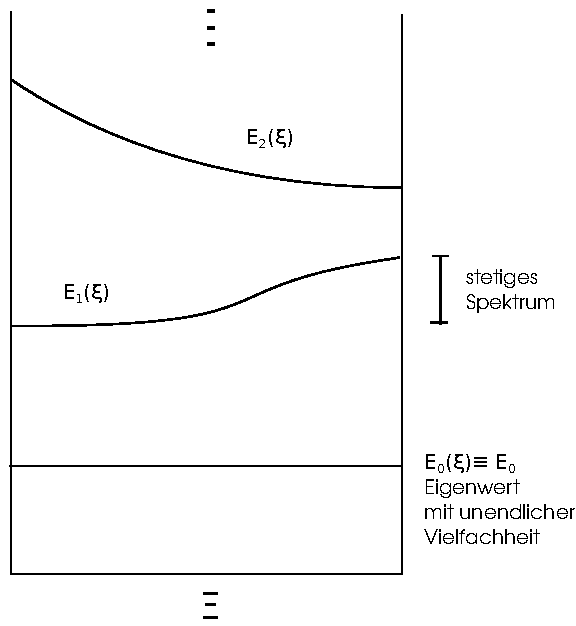
\includegraphics[width=0.4 \textwidth]{energiespektren.pdf}
\caption{Das Spektrum ergibt sich gerade als Vereinigung der Eigenwerte der jeweiligen Energiespektren der Zerlegung.}
\end{figure}

\begin{thebibliography}{tief}
\bibitem{1} Reed-Simon: {\it Methods of Modern Mathematical Physics}. Volume 4. Academic Press, Inc., 1978.
\end{thebibliography} 

\end{document}
